Para la primera parte implementamos la tarea \textbf{TaskConsola}, la cual simula ser una tarea interactiva.

TaskConsola recibe tres parámetros: $n$, $bmin$ y $bmax$; y debe realizar $n$ llamadas bloqueantes, cada una con un tiempo pseudoaleatorio entre $bmin$ y $bmax$. 

Con el fin de generar este tiempo debimos generar un número pseudoaleatorio $random\_number$, para lo cual utilizamos las funciones rand() y srand($seed$) definidas en la stdlib. El número es generado por rand() dentro del rango [0..RAND\_MAX] bajo una semilla introducida por srand($seed$) donde $seed$ la calculamos en función del horario en el cual corre la tarea ($\#include <sys/time.h>$). Vale aclarar que $RAND\_MAX$ asumimos menor o igual a 32767, el valor estándar. Es una constante definida en <cstdlib>.

Luego, el tiempo $t$ para la i-ésima llamada bloqueante es dado por la siguiente operación:

\begin{center}
	$t = bmin + (random\_number \ \% \ (bmax-bmin+1))$
\end{center}

%{\centering
%	$t = bmin + (random\_number \ \% \ (bmax-bmin+1))$
%
%}

De ese modo el tiempo $t$ se encuentra efectivamente dentro del intervalo deseado (entre $bmin$ y $bmax$ inclusive).

\subsection{SchedFCFS}

Luego implementamos el scheduler \textbf{SchedFCFS}, que utiliza el algoritmo de First-Come First-Served. Dicho de otro modo, las tareas se ejecutan por órden de llegada y hasta que finalice su ejecución. Implementamos el SchedFCFS sobre una cola de tareas en estado $ready$, donde la función LOAD se resume en simplemente encolar el pid de la tarea a cargar; la función UNBLOCK no tiene uso dado que aún si la tarea se bloquea, esta corre en el cpu hasta que finalice su espera; y la función TICK simplemente cambia de tarea cuando se la llama con motivo de exit y la tarea que corría en el cpu termina.

~

A continuación un gráfico del comportamiento del SchedFCFS con uno, dos y tres cores, sin costos de migración o cambio de contexto, para un lote de 3 tareas, dos interactivas TaskConsola y una TaskCPU de procesamiento intensivo.

\begin{figure}[H]
\centering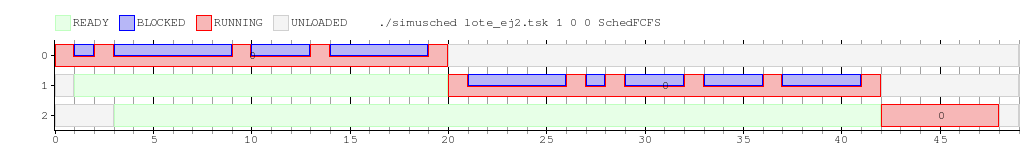
\includegraphics[width=18 cm]{graficos/ej2FCFS1.png}
\centering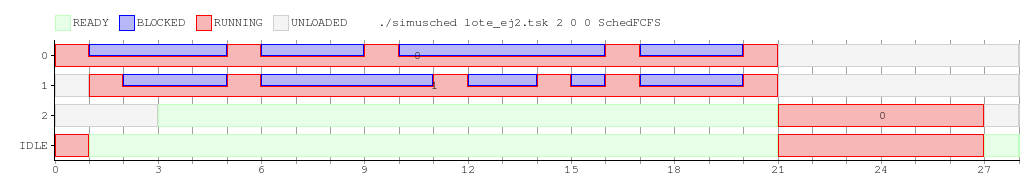
\includegraphics[width=18 cm]{graficos/ej2FCFS2.png}
\centering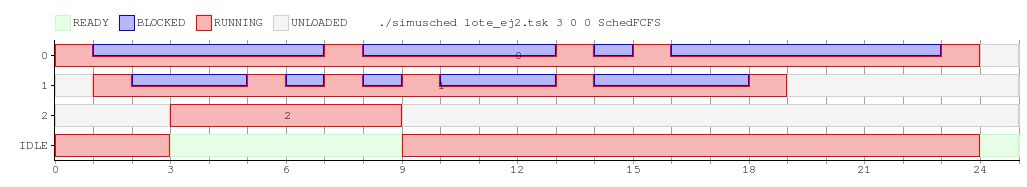
\includegraphics[width=18 cm]{graficos/ej2FCFS3.png}
\caption{First-Come First-Served, un sólo núcleo de procesamiento en el primer caso, dos en el segundo y por último tres núcleos.}
\end{figure}

Podemos ver en la figura 1 que, si bien este algoritmo evita posibles costosos cambios de contexto y costos de migración, se pierde mucha interactividad. Con un único núcleo la tarea TaskCPU debe esperar a las dos tareas bloqueantes para finalmente correr, cuando podría haber terminado si esta corría mientras las interactivas permanecían bloqueadas.

Lo mismo sucede en el segundo caso, pero desde ya al correr las TaskConsola en paralelo, esto acorta considerablemente el tiempo de espera de la tarea intensiva en CPU. Luego las tres tareas en paralelo permiten con este algoritmo ahorrar en cambios de contexto o migración, ya que otro algoritmo podrìa rotar a las tareas entre los núcleos.



